Bevor die Anfangswerte zur globalen Beleuchtung benutzt werden(siehe auch \nameref{pic:Render Graph}), durchlaufen Sie nach dem Sortieren 
\ref{ch:Content2:sec:Sorting} das Retargeting. Der Sinn liegt hierbei beim Vertauschen der Anfangswerte, sodass Sie 
verteilt sind wie $BlueNoise_{t}$ , aufgrund des zuvor ausgeführten Sortierschrittes \ref{ch:Content2:sec:Sorting},
sodass Sie verteilt sind wie die Textur $BlueNoise_{t+1}$. Aufgrund dessen haben wir eine Aufsummierung der
\nameref{ch:Content1:sec:blue noise} Fehlerverteilungen über die ersten paar Bilder(siehe \nameref{fig:Retargeting_And_Sorting_Szene_t1}).

\begin{figure}[H]

    %%%%%%%%%%%%%%%%%%%%%%%%%%%%%%%%%%%%%%%%%%%%%%%%%%%%%%%%%%%%%%%%%%%%%%%%%%%%%%%%%%%%%%%%%%%%%%%%%%%%%%
    %%%%%%%%%%%%%%%%%%%%%%%%%%%%%%% second row --> sorting block size 2 without retargeting
    %%%%%%%%%%%%%%%%%%%%%%%%%%%%%%%%%%%%%%%%%%%%%%%%%%%%%%%%%%%%%%%%%%%%%%%%%%%%%%%%%%%%%%%%%%%%%%%%%%%%%%

    \centering
    \begin{subfigure}[b]{0.2\linewidth}
      
\includegraphics[width=\linewidth]{content/TemporalerAlg/Bilder/Retargeting/Bedeutung Retargeting/SortSerie/seed_debug_3.0_small.png}
       \caption{FT t = 0}
       \label{pic:sortier_t0}
    \end{subfigure}
    \begin{subfigure}[b]{0.2\linewidth}
      
\includegraphics[width=\linewidth]{content/TemporalerAlg/Bilder/Retargeting/Bedeutung Retargeting/SortSerie/seed_debug_4.0_small.png}
      \caption{FT t = 1}
      \label{pic:sortier_t1}
    \end{subfigure}
    \begin{subfigure}[b]{0.2\linewidth}
      
\includegraphics[width=\linewidth]{content/TemporalerAlg/Bilder/Retargeting/Bedeutung Retargeting/SortSerie/seed_debug_5.0_small_screen.png}
      \caption{Ausschnitt t=2}
      \label{pic:sortier_screen_t2}
    \end{subfigure}
    \begin{subfigure}[b]{0.2\linewidth}
        
\includegraphics[width=\linewidth]{content/TemporalerAlg/Bilder/Retargeting/Bedeutung Retargeting/SortSerie/seed_debug_5.0_small.png}
        \caption{FT t = 2}
        \label{pic:sortier_t2}
      \end{subfigure}
    
    %%%%%%%%%%%%%%%%%%%%%%%%%%%%%%%%%%%%%%%%%%%%%%%%%%%%%%%%%%%%%%%%%%%%%%%%%%%%%%%%%%%%%%%%%%%%%%%%%%%%%%
    %%%%%%%%%%%%%%%%%%%%%%%%%%%%%%% second row --> sorting block size 2 with retargeting
    %%%%%%%%%%%%%%%%%%%%%%%%%%%%%%%%%%%%%%%%%%%%%%%%%%%%%%%%%%%%%%%%%%%%%%%%%%%%%%%%%%%%%%%%%%%%%%%%%%%%%%

    \begin{subfigure}[b]{0.2\linewidth}
        
\includegraphics[width=\linewidth]{content/TemporalerAlg/Bilder/Retargeting/Bedeutung Retargeting/RetargetSerie/seed_debug_3.0_small.png}
         \caption{FT t = 0}
         \label{pic:retarget_t0}
    \end{subfigure}
    \begin{subfigure}[b]{0.2\linewidth}
        
\includegraphics[width=\linewidth]{content/TemporalerAlg/Bilder/Retargeting/Bedeutung Retargeting/RetargetSerie/seed_debug_4.0_small.png}
         \caption{FT t = 1}
         \label{pic:retarget_t1}
    \end{subfigure}
    \begin{subfigure}[b]{0.2\linewidth}
        
\includegraphics[width=\linewidth]{content/TemporalerAlg/Bilder/Retargeting/Bedeutung Retargeting/RetargetSerie/seed_debug_5.0_small_screen.png}
         \caption{Ausschnitt t=2}
         \label{pic:retarget_screen_t2}
    \end{subfigure}
    \begin{subfigure}[b]{0.2\linewidth}
        
\includegraphics[width=\linewidth]{content/TemporalerAlg/Bilder/Retargeting/Bedeutung Retargeting/RetargetSerie/seed_debug_5.0_small.png}
         \caption{FT t = 2}
         \label{pic:retarget_t2}
    \end{subfigure}
    \caption{Vergleich erste Bilder Sorting(B=2) mit bzw. ohne Retargeting}
    \label{fig:VergleichRetargetSorting}
      
\end{figure}

Die Abbildung \ref{fig:VergleichRetargetSorting} verdeutlicht die Bedeutung des Retargeting 
Schrittes.

\begin{algorithm}[H]
    \caption{\textbf{Retargeting Schritt}}
    \begin{algorithmic}[1]
        \State //permutation indices from precomputed texture
        \State $retaget_{t}$ = retarget\_texure[calc\_correct\_offset()];
        
        \State $retargetedSeeds(old\_id + retaget_{t}) = incomingSeeds(old\_id);$
        
    \end{algorithmic}
    \label{alg:retargetingAlg}
\end{algorithm}

\begin{figure}[H]\label{pic:Permutation}
    \centering
    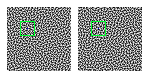
\includegraphics[width=0.5\linewidth]{content/simulatedAnnealing/Bilder/Permutation.png}
    \caption{Permutation}
\end{figure}

\begin{algorithm}[H]
    \caption{Benutzung unser zwei vorberechneten Texturen: Blue Noise und Retarget}
    \begin{algorithmic}[1]
        \State $bluenoise_{t}$(i,j) = $bluenoise_{0}$(i + $\alpha$t, j + $\beta$t); 
        \State $retarget_{t}$(i,j) = $retarget_{0}$(i + $\alpha$t, j + $\beta$t) + ($\alpha$t, $\beta$t)
    \end{algorithmic}
    \label{alg:Benutzung vorberechneter Texturen}
\end{algorithm}

\newpage
%%%%%%%%%%%%%%%%%%%%%%%%%%%%%%%%%%%%%%%%%%%%%%%%%%%%%%%%%%%%
%%%%%%%%%% Beginning the Sequence of getting to blue noise from white noise
%%%%%%%%%%%%%%%%%%%%%%%%%%%%%%%%%%%%%%%%%%%%%%%%%%%%%%%%%%%%
\label{fig:Retargetbilderstrecke}
\begin{figure}[H]

    \begin{subfigure}{\textwidth}
        \centering 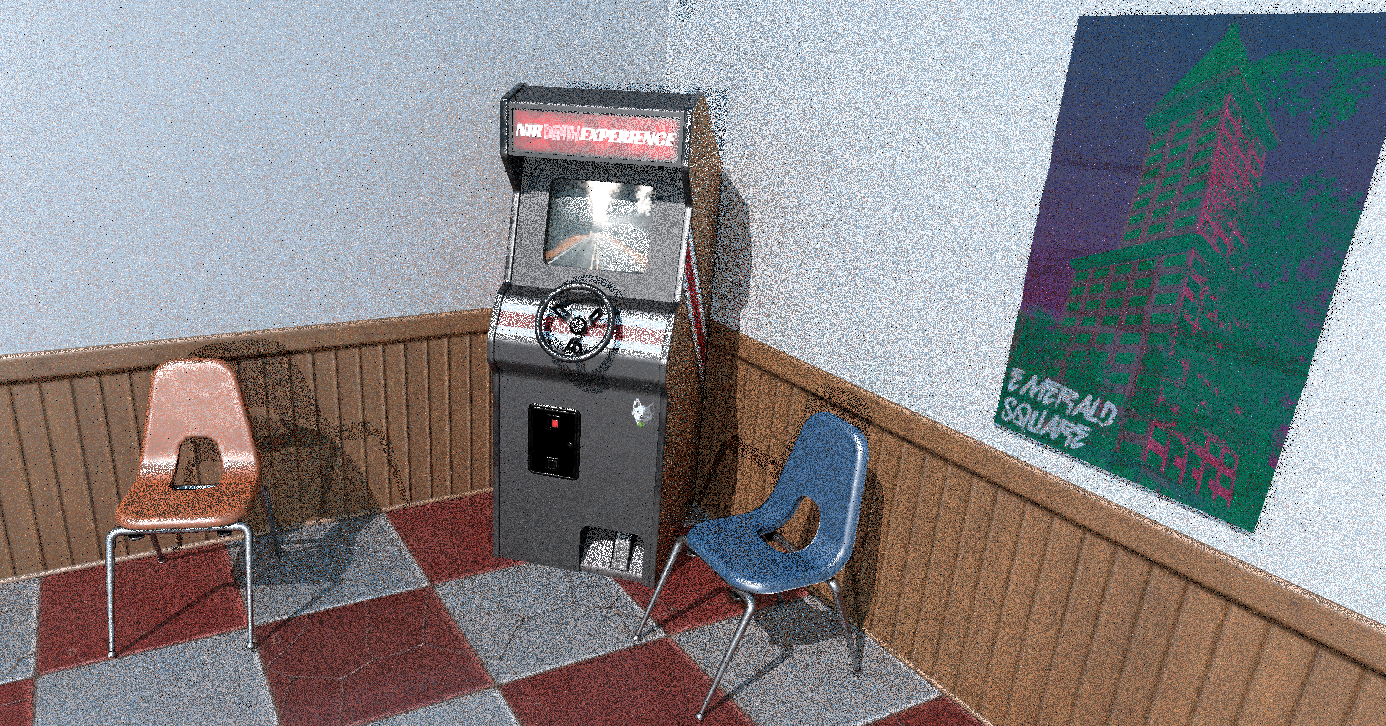
\includegraphics[scale=.25]{content/TemporalerAlg/Bilder/Retargeting/Screenshots/seed_debug_3.0_selection.png}
        \caption{Szene}
        \label{fig:Retargeting_And_Sorting_Szene_t1}
    \end{subfigure}
    \begin{subfigure}{0.5\textwidth}
        \centering 
\includegraphics[width=0.4\linewidth]{content/TemporalerAlg/Bilder/Retargeting/Screenshots/seed_debug_3.0_ausschnitt.png} 
        \caption{Szenenausschnitt}
        \label{fig:Retargeting_And_Sorting_ausschnitt_t1}
    \end{subfigure}
    \begin{subfigure}{0.5\textwidth}
        \centering 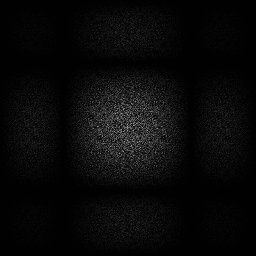
\includegraphics[width=0.4\linewidth]{content/TemporalerAlg/Bilder/Retargeting/Screenshots/Spektren/seed_debug_3.0_ausschnitt.png}
        \caption{Fouriertransformierte des Ausschnitts}
        \label{fig:Retargeting_And_Sorting_Fouriertransformierte_t1}
    \end{subfigure}
        \caption{Zeitpunkt t=1}
        \label{fig:Retargeting_And_Sorting_Verlauf_t1}
\end{figure}

\begin{figure}[H]
    \begin{subfigure}{\textwidth}
        \centering 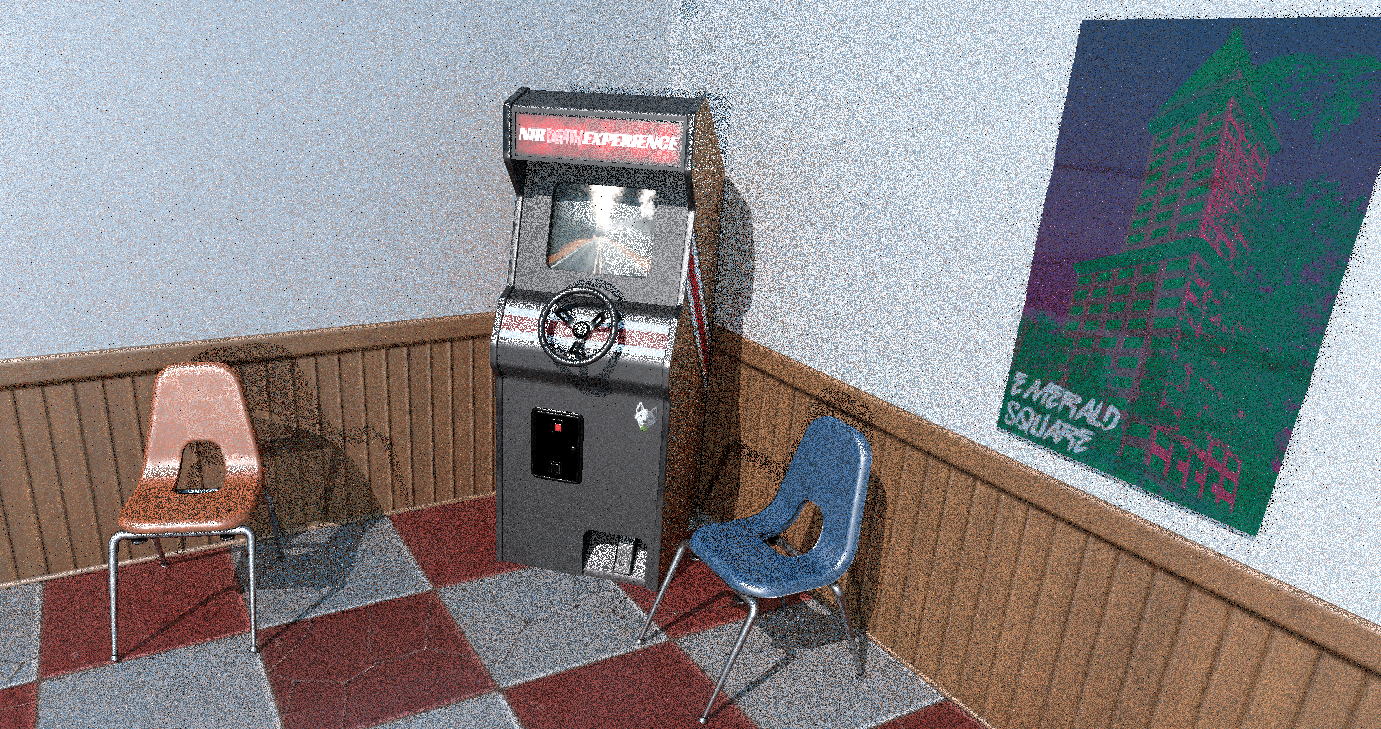
\includegraphics[scale=.25]{content/TemporalerAlg/Bilder/Retargeting/Screenshots/seed_debug_4.0_selection.png}
        \caption{Szene}
        \label{fig:Retargeting_And_Sorting_Szene_t2}
    \end{subfigure}
    \begin{subfigure}{0.5\textwidth}
        \centering
\includegraphics[width=0.4\linewidth]{content/TemporalerAlg/Bilder/Retargeting/Screenshots/seed_debug_4.0_ausschnitt.png} 
        \caption{Szenenausschnitt}
        \label{fig:Retargeting_And_Sorting_ausschnitt_t2}
    \end{subfigure}
    \begin{subfigure}{0.5\textwidth}
        \centering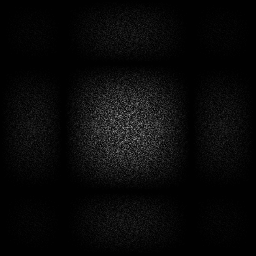
\includegraphics[width=0.4\linewidth]{content/TemporalerAlg/Bilder/Retargeting/Screenshots/Spektren/seed_debug_4.0_ausschnitt.png}
        \caption{Fouriertransformierte des Ausschnitts}
        \label{fig:Retargeting_And_Sorting_Fouriertransformierte_t2}
    \end{subfigure}
        \caption{Zeitpunkt t=2}
        \label{fig:Retargeting_And_Sorting_Verlauf_t2}
\end{figure}

\begin{figure}[H]
    \begin{subfigure}{\textwidth}
        \centering 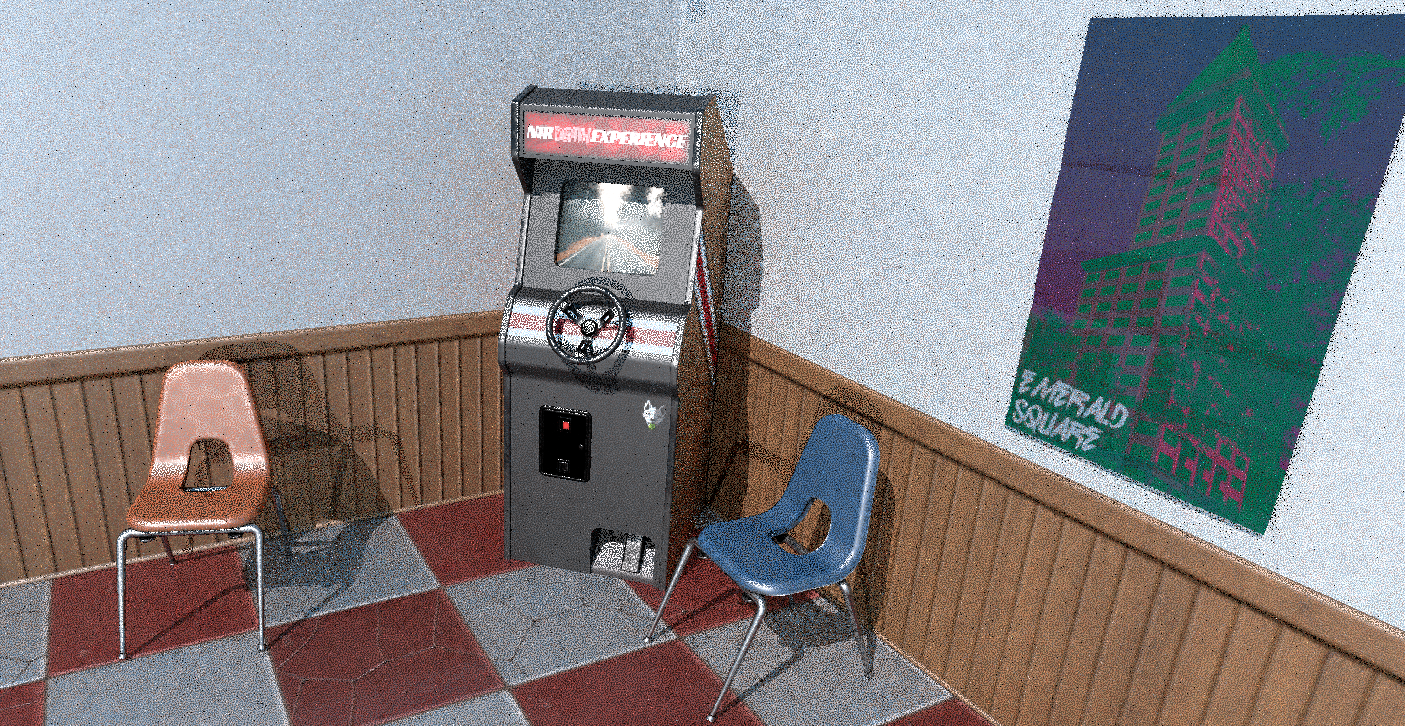
\includegraphics[scale=.25]{content/TemporalerAlg/Bilder/Retargeting/Screenshots/seed_debug_5.0_selection.png}
        \caption{Szene}
        \label{fig:Retargeting_And_Sorting_Szene_t3}
    \end{subfigure}
    \begin{subfigure}{0.5\textwidth}
        \centering
\includegraphics[width=0.4\linewidth]{content/TemporalerAlg/Bilder/Retargeting/Screenshots/seed_debug_5.0_ausschnitt.png} 
        \caption{Szenenausschnitt}
        \label{fig:Retargeting_And_Sorting_ausschnitt_t3}
    \end{subfigure}
    \begin{subfigure}{0.5\textwidth}
        \centering
\includegraphics[width=0.4\linewidth]{content/TemporalerAlg/Bilder/Retargeting/Screenshots/Spektren/seed_debug_5.0_ausschnitt.png}
        \caption{Fouriertransformierte des Ausschnitts}
        \label{fig:Retargeting_And_Sorting_Fouriertransformierte_t3}
    \end{subfigure}
        \caption{Zeitpunkt t=3}
        \label{fig:Retargeting_And_Sorting_Verlauf_t3}
\end{figure}

\begin{figure}[H]
    \begin{subfigure}{\textwidth}  
        \centering 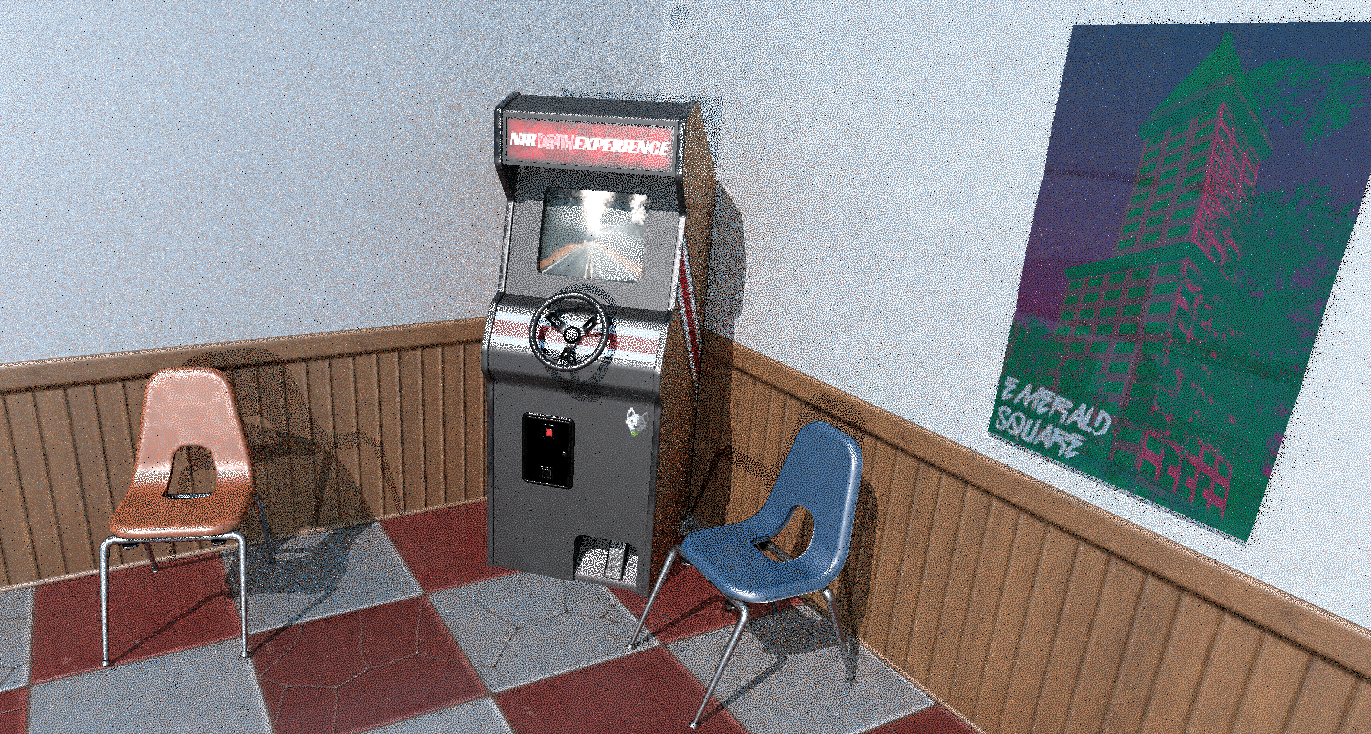
\includegraphics[scale=.25]{content/TemporalerAlg/Bilder/Retargeting/Screenshots/seed_debug_6.0_selection.png}
        \caption{Szene}
        \label{fig:Retargeting_And_Sorting_Szene_t4}
    \end{subfigure}
    \begin{subfigure}{0.5\textwidth}
        \centering
\includegraphics[width=0.4\linewidth]{content/TemporalerAlg/Bilder/Retargeting/Screenshots/seed_debug_6.0_ausschnitt.png} 
        \caption{Szenenausschnitt}
        \label{fig:Retargeting_And_Sorting_ausschnitt_t4}
    \end{subfigure}
    \begin{subfigure}{0.5\textwidth}
        \centering
\includegraphics[width=0.4\linewidth]{content/TemporalerAlg/Bilder/Retargeting/Screenshots/Spektren/seed_debug_6.0_ausschnitt.png}
        \caption{Fouriertransformierte des Ausschnitts}
        \label{fig:Retargeting_And_Sorting_Fouriertransformierte_t4}
    \end{subfigure}
        \caption{Zeitpunkt t=4}
        \label{fig:Retargeting_And_Sorting_Verlauf_t4}
\end{figure}

\begin{figure}[H]
    \begin{subfigure}{\textwidth}   
        \centering 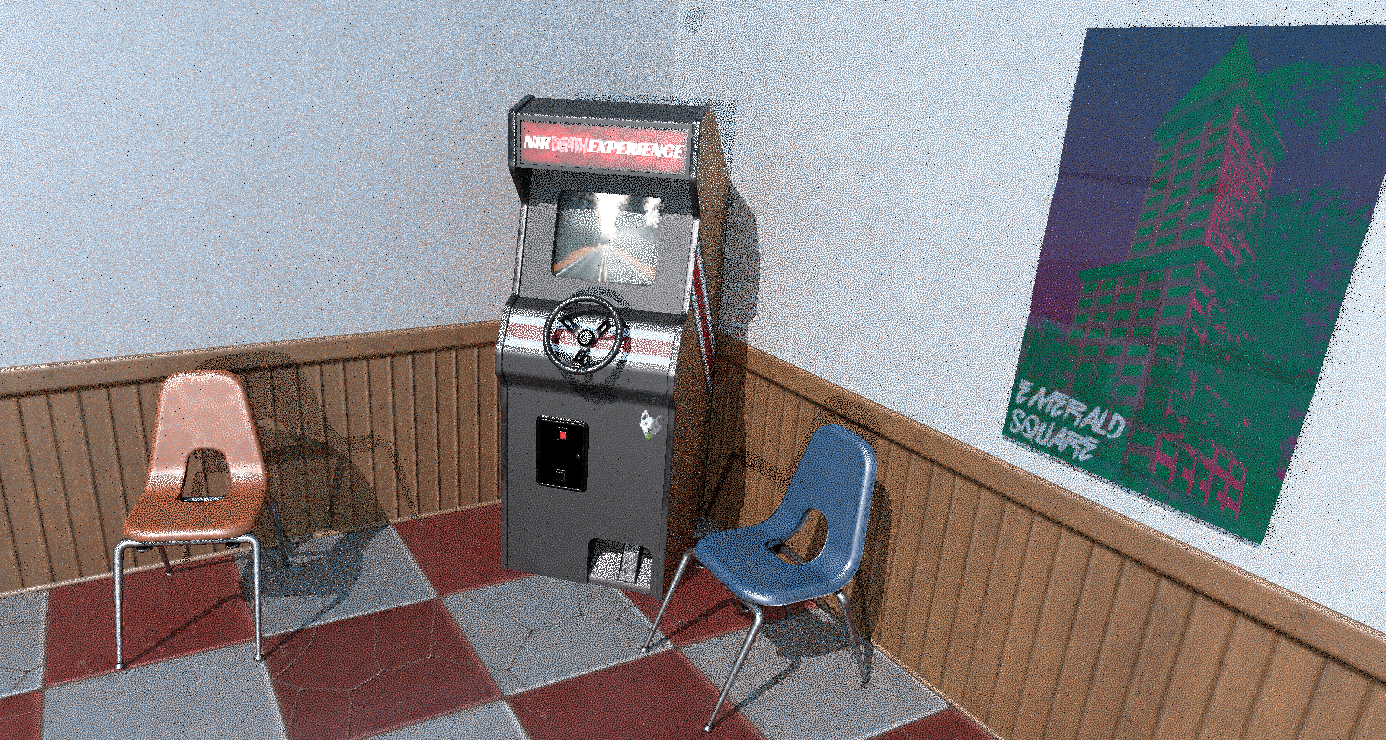
\includegraphics[scale=.25]{content/TemporalerAlg/Bilder/Retargeting/Screenshots/seed_debug_7.0_selection.png}
        \caption{Szene}
        \label{fig:Retargeting_And_Sorting_Szene_t5}
    \end{subfigure}
    \begin{subfigure}{0.5\textwidth}
        \centering
\includegraphics[width=0.4\linewidth]{content/TemporalerAlg/Bilder/Retargeting/Screenshots/seed_debug_7.0_ausschnitt.png} 
        \caption{Szenenausschnitt}
        \label{fig:Retargeting_And_Sorting_ausschnitt_t5}
    \end{subfigure}
    \begin{subfigure}{0.5\textwidth}
        \centering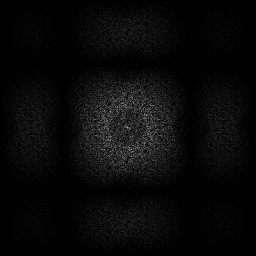
\includegraphics[width=0.4\linewidth]{content/TemporalerAlg/Bilder/Retargeting/Screenshots/Spektren/seed_debug_7.0_ausschnitt.png}
        \caption{Fouriertransformierte des Ausschnitts}
        \label{fig:Retargeting_And_Sorting_Fouriertransformierte_t5}
    \end{subfigure}
        \caption{Zeitpunkt t=5}
        \label{fig:Retargeting_And_Sorting_Verlauf_t5}
\end{figure}

\begin{figure}[H]
    \begin{subfigure}{\textwidth}   
        \centering 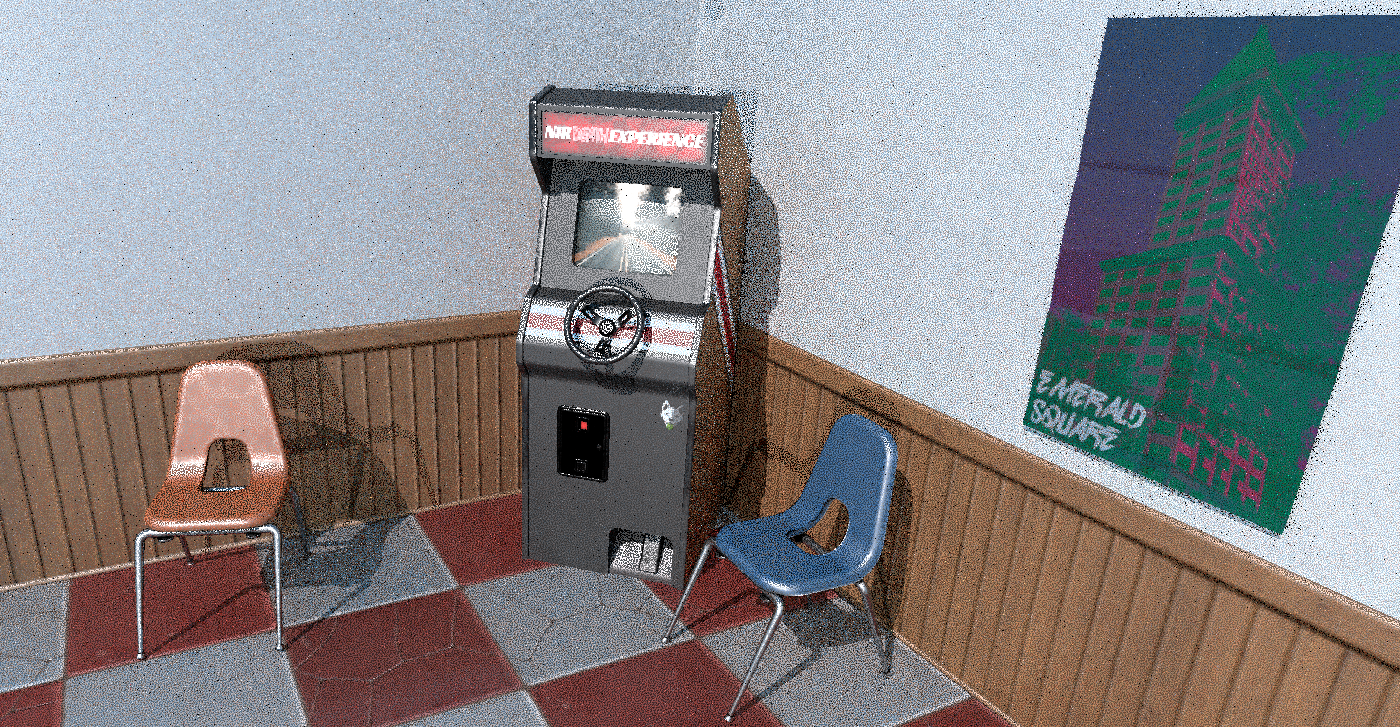
\includegraphics[scale=.25]{content/TemporalerAlg/Bilder/Retargeting/Screenshots/seed_debug_8.0_selection.png}
        \caption{Szene}
        \label{fig:Retargeting_And_Sorting_Szene_t6}
    \end{subfigure}
    \begin{subfigure}{0.5\textwidth}
        \centering
\includegraphics[width=0.4\linewidth]{content/TemporalerAlg/Bilder/Retargeting/Screenshots/seed_debug_8.0_ausschnitt.png} 
        \caption{Szenenausschnitt}
        \label{fig:Retargeting_And_Sorting_ausschnitt_t6}
    \end{subfigure}
    \begin{subfigure}{0.5\textwidth}
        \centering
\includegraphics[width=0.4\linewidth]{content/TemporalerAlg/Bilder/Retargeting/Screenshots/Spektren/seed_debug_8.0_ausschnitt.png}
        \caption{Fouriertransformierte des Ausschnitts}
        \label{fig:Retargeting_And_Sorting_Fouriertransformierte_t6}
    \end{subfigure}
        \caption{Zeitpunkt t=6}
        \label{fig:Retargeting_And_Sorting_Verlauf_t6}
\end{figure}

\begin{figure}[H]
    \begin{subfigure}{\textwidth}   
        \centering 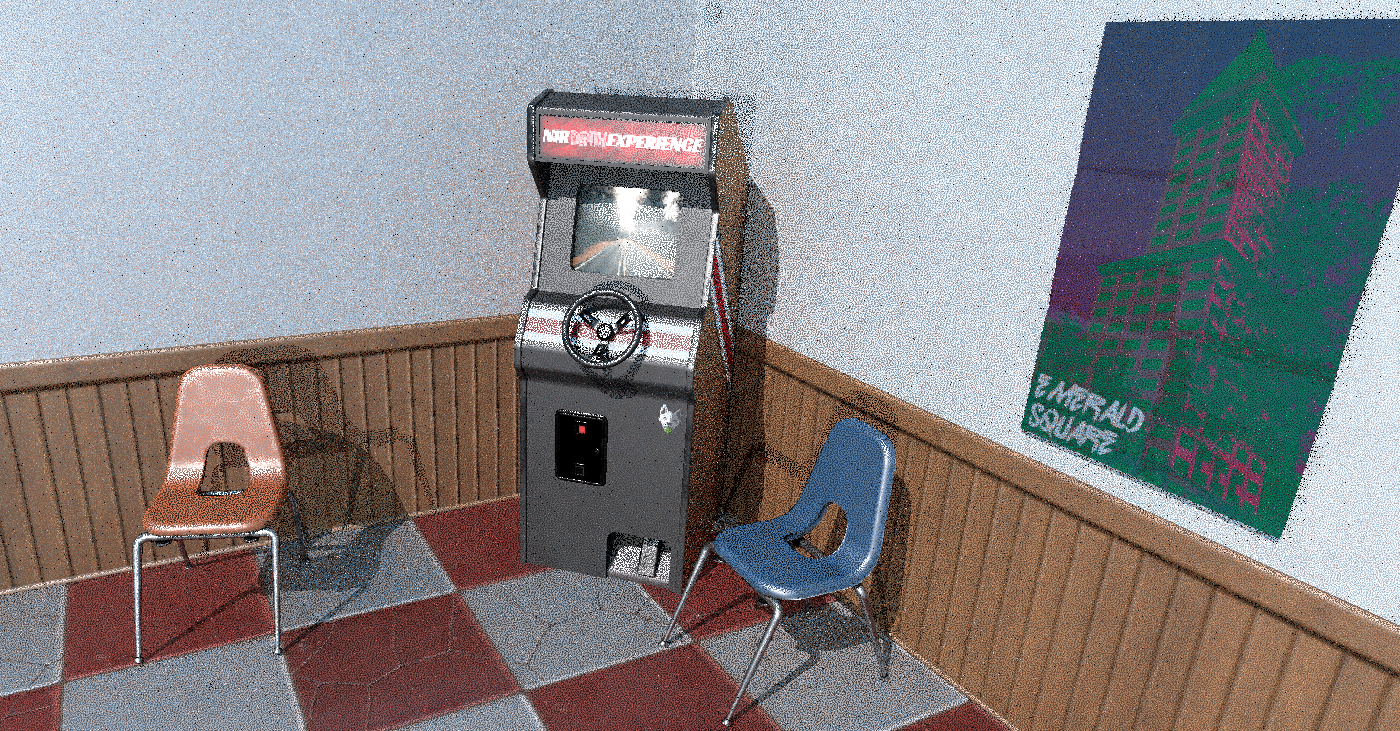
\includegraphics[scale=.25]{content/TemporalerAlg/Bilder/Retargeting/Screenshots/seed_debug_9.0_selection.png}
        \caption{Szene}
        \label{fig:Retargeting_And_Sorting_Szene_t7}
    \end{subfigure}
    \begin{subfigure}{0.5\textwidth}
        \centering
\includegraphics[width=0.4\linewidth]{content/TemporalerAlg/Bilder/Retargeting/Screenshots/seed_debug_9.0_ausschnitt.png} 
        \caption{Szenenausschnitt}
        \label{fig:Retargeting_And_Sorting_ausschnitt_t7}
    \end{subfigure}
    \begin{subfigure}{0.5\textwidth}
        \centering
\includegraphics[width=0.4\linewidth]{content/TemporalerAlg/Bilder/Retargeting/Screenshots/Spektren/seed_debug_9.0_ausschnitt.png}
        \caption{Fouriertransformierte des Ausschnitts}
        \label{fig:Retargeting_And_Sorting_Fouriertransformierte_t7}
    \end{subfigure}
        \caption{Zeitpunkt t=7}
        \label{fig:Retargeting_And_Sorting_Verlauf_t7}
\end{figure}

